%!TEX root = ../../../../thesis.tex
\section{Introduction to Myxomycetes and Physarum Polycephalum}

In this section we give a basic introduction to slime molds and \P in particular. We summarize selected material form several sources that provide more detailed surveys~\cite{nowotny2000myxomyceten,grube2016physarum,Sauer1986,Mayne2016,howard1931life}. Our exposition closely follows~\cite{nowotny2000myxomyceten}.

\subsection{Life of Slime}

The life cycle of \P starts with its spores which are propagated in a predominately airborne fashion. After an incubation period of a few days, spores begin to germinate in favorable conditions. Soon the walls of the spores break open to release haploid protoplasmic bodies of $12-15 \mu m$ in diameter. After a short period of quiescence these so-called myxoamoebae become active to grow and multiply like other soil amoebae. 

Two reversible processes illustrate the remarkable adaptability of \P myxoamoebae. First, they have the ability to quickly grow one or two flagellae, \ie change into myxoflagellates, to better navigate moist environments such as water films. Furthermore, both types of myxoamoebae are able to form dormant micro cysts capable of enduring adverse conditions such as dryness or strong illumination. As soon as conditions become favorable again, myxoabmoebae escapte their cysts and are ready to continue the life cycle.

Next, pairwise sexual or heterothallic fusion between two haploid myxoamoeba lead to the irreversible formation of a diploid zygote. It is also possible that a single myxoamoeba changes directly into a haploid zygote in an apogamic or selfing fashion.

Both types of zygotes have in common that from now on nuclear division happens synchronously every $8-10$ hours without cell devision. This dramatic change signals the onset of a peculiar cellular organization, the so-called \emph{plasmodium}. In this stage \P lives as an macroscopic slimy mass of protoplasm consisting of up to millions of nuclei contained in a singular cell. Remarkably, the plasmodium stage is unique to myxomycetes and unparalleled throughout Nature.

In its plasmodium stage \P is acting as an undifferentiated macroscopic creature, capable of sensing food sources, migrating towards them and feeding on them by means of phagozytosis. Typical food sources encountered by \P in the field include bacteria, amoebae, algae, common molds and various organic materials. It is also known to feed on spores, hypen or fruting bodies of higher fungi. In the lab \P can sustain itself on substrates containing solute nutrients. Under continued food intake, the plasmodium can grow to cover large areas of up to  several $dm^2$. Under unfavorable conditions the plasmodium can change into many multinucleated dormant macrozysts, forming a crust of dried slime, the so-called \emph{sclerotium}. \P may reverse back to its plasmodium form in better conditions even after long periods of lying dormant.

Towards the end of the life cycle, triggered by lillumination, the plasmodium seeks out dry and preferably elevated locations to begin the irreversible process of sporulation. In a synchronus differentiation procees \P forms colonies of $1-2$ mm tall fruiting bodies. These so-called sporangia are numerous and come with a stem and a head each. Their appearance inspired the species designation \Pp, the multiheaded. Within the fruiting bodies spores, responsible for species propagation, are maturing. When mature they are dispersed by the wind and the life cycle of \P, given suitable conditions, starts anew.

It is fascinating how this multipotent development system exists in extremely different forms of live while controlled by one and the same genome in a unique temporal sequence. From spores to amoeba, on to plasmodium and finally to fruiting bodies. From there back to spores and again into more amoeba. The complete life cycle of \Pp is illustrated in \Fref{fig:life_cycle}.

\begin{figure}[ht]
	\centering
	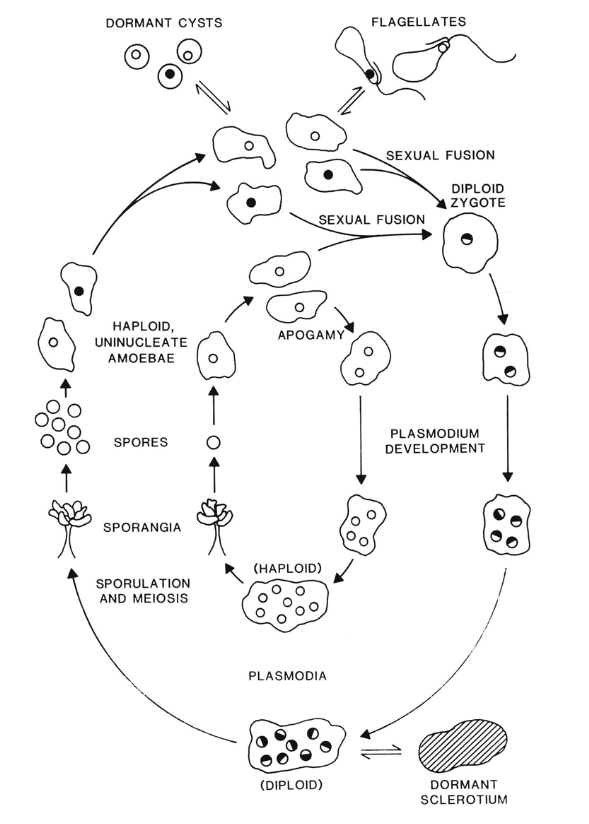
\includegraphics[width=\textwidth,height=0.9\textheight,keepaspectratio]{life_cycle.png}
	\caption[Life cycle of \P]{The complete life cycle of \Pp. Reprint from~\cite{Sauer1986}.}
	\label{fig:life_cycle}
\end{figure}


\subsection{The plasmodium stage}

\subsection{Research on Physarum}

